\begin{frame}
  \frametitle{}
\end{frame}

\begin{frame}
  \frametitle{}
\end{frame}

\begin{frame}
  \frametitle{}
\end{frame}

\begin{frame}[fragile]
  \frametitle{三目运算}
  \begin{itemize}
    \item 三目运算语法格式:
     \java|x ? y : z|
    \item 解释:其中\texttt{x}为布尔型类型的表达式,如果\texttt{x}为真,则返回\texttt{y};否则,返回\texttt{z}
  \end{itemize}
  
  \begin{javacode}
  int score = 80;
  String type = score > 60 ? "及格" : "不及格"; 
  
  int x = -1;
  int flag =  x > 0 ? 1 : (x == 0 ? 0 : -1)
  \end{javacode}

\end{frame}

\begin{frame}
  \frametitle{语句}
  \begin{itemize}
    \item 条件语句:根据不同条件,执行不同的代码块
      \java|if|
      \java|if ... else ...|
      \java|if ... else if ... else ...|
      \java|switch ... case ... case ... default ...|
    \item 循环语句:当满足某条件时,重复执行代码块
      \java |for|
      \java |while|
      \java |do ... while ...|
  \end{itemize}

\end{frame}

\begin{frame}[fragile]
  \frametitle{条件语句}
    \begin{columns}
      \column{0.4\textwidth}
        \begin{javacode*}{label=IF语句}
       if (x) {
       
       } 
       
       if (x) {
       
       } else {
       
       }
       
       if (x) {
       
       } else if (y) {
       
       } else {
       
       }
      \end{javacode*}
      \column{0.6\textwidth}
      \begin{javacode*}{label=Switch语句}
        switch(参数) {
          //如果“参数”的值等于“常量表达式1”,则执行
          case 常量表达式1: 
            ...
            break; 
            //不要忘记加break,否则会有副作用
          case 常量表达式2: 
            ...
            break;
          default: 
            break;
        }
      \end{javacode*}
      \begin{itemize}
        \item 小心\texttt{case}穿透,注意加上必要的\texttt{break}
        \item default可以省略,单不推荐
      \end{itemize}
    \end{columns}
\end{frame}


\begin{frame}[fragile]
  \frametitle{FOR循环语句}
  \begin{javacode*}{label=传统形式}
    int[] arr = new int[]{1, 2, 3, 4};
    
    for (int i=0; i< arr.length; i++) {
      System.out.println(x);
    }
  \end{javacode*}
  
  \begin{javacode*}{label=Java 5.0增强形式}
    for (int x in arr) {
      System.out.println(x);
    }
  \end{javacode*}
\end{frame}

\begin{frame}[fragile]
  \frametitle{WHILE循环}
  \begin{columns}
      \column{0.5\textwidth}
        \begin{javacode*}{label=WHILE语句}
          while (逻辑表达式1) {
            代码块1
          }
          //最后没有分号
        \end{javacode*}
        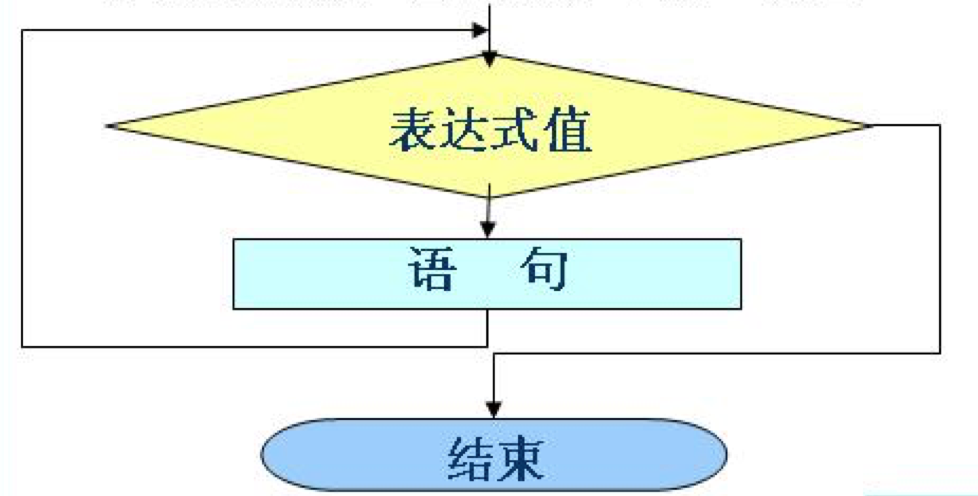
\includegraphics[width=\textwidth, height=80pt]{figures/while}
        当不满足“逻辑表达式1”时,“代码块1”一次都不会执行!
      \column{0.5\textwidth}
        \begin{javacode*}{label=DO WHILE语句}
          do {
            代码块2
          } while (逻辑表达式2); 
          //不要忘记最后有分号
        \end{javacode*}
        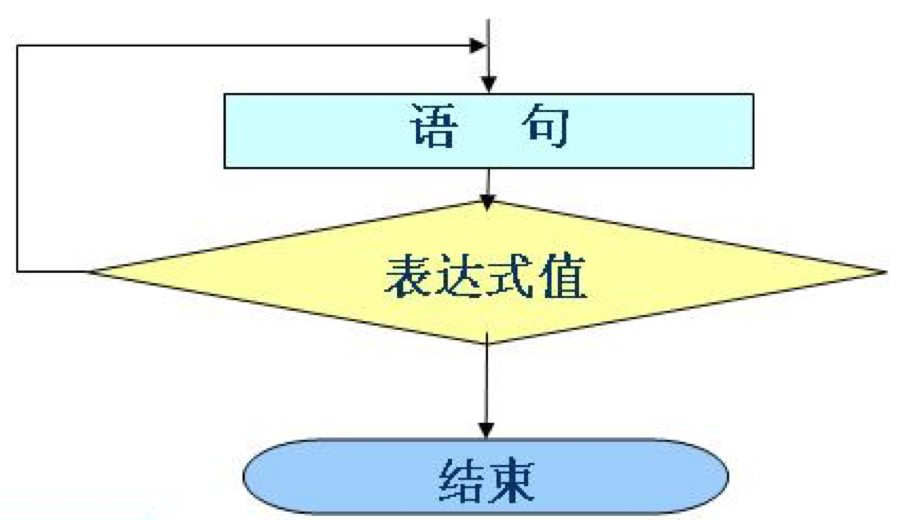
\includegraphics[width=\textwidth, height=80pt]{figures/do_while}
        当不满足“逻辑表达式2”时,“代码块2”会执行1次!
  \end{columns}
    
  \center{如果没有特殊需求,请用第一种WHILE语句!因为第一种WHILE语句意思更明了,更易理解,更加不容易出现副作用!}
\end{frame}

\begin{frame}[fragile]
  \frametitle{循环控制:break语句和continue语句}
    \begin{columns}
      \column{0.5\textwidth}
        break语句用于提前终止循环体的执行,可以强制退出循环,并且不再进行下一轮循环的判定和执行
        \begin{javacode}
        for (int i=0; i< arr.length; i++) { //arr是[1,2,3,4]
          if (i == 3) {
            break;//跳出本循环
          }
          System.out.println(x);
        }
        //只会打印“1, 2”!
        \end{javacode}
      \column{0.5\textwidth}
        continue语句可以提前终止本次循环体的执行,不再执行该语句后面的循环体,开始下一轮循环的判定和执行
        \begin{javacode}
        for (int i=0; i< arr.length; i++) {//arr是[1,2,3,4]
          if (i == 3) {
            continue;//跳出本轮循环
          }
          System.out.println(x);
        }
        //会打印“1, 2, 4”, 不会打印“3”!
        \end{javacode}   
  \end{columns}
  \center{
  \begin{itemize}
    \item 相同点:立即退出本轮循环的循环体,后续循环体的语句都不执行
    \item 不同点:break语句不再进入下一轮的循环判定,而continue语句会进入下一轮的循环判定
  \end{itemize}
  }

\end{frame}

\begin{frame}
  \frametitle{迭代(recursion)}
  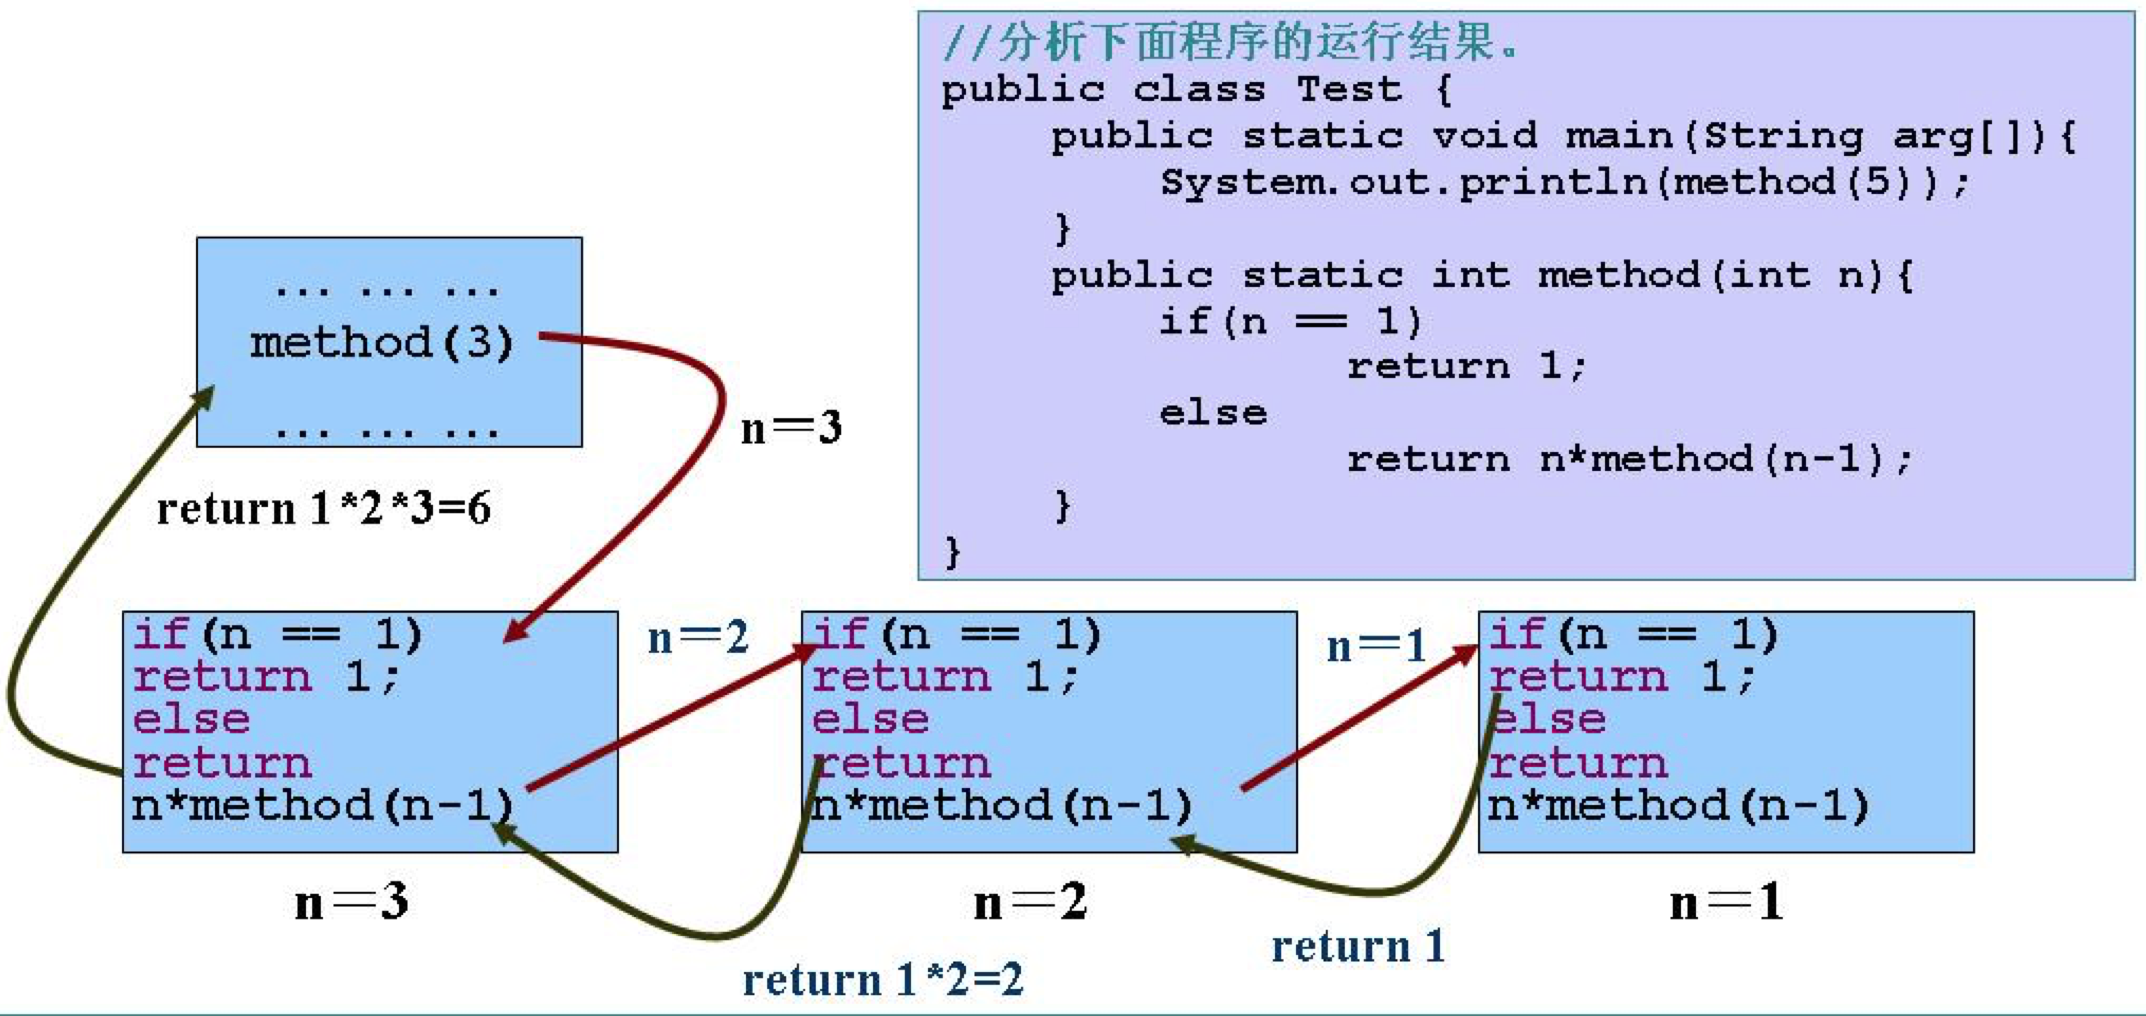
\includegraphics[width=\textwidth]{figures/recursion}
\end{frame}
